% p19-strict-curry-and-strict-apply-commute.tex
%
% Source:   Carl A. Gunter and Dana S. Scott, "Semantic Domains".
%           ScottDomains/papers/Gunter Scott 1990.pdf
% Physical page: 19          Printed page: 18
% Section:  4.3 Smash products.
% Unnamed in the paper (no figure number). Introduced by:
%   "In particular, there is a strict continuous function strict_apply such
%    that for any strict function f, there is a unique strict function
%    strict_curry such that the following diagram commutes:"
%
% Content: a commutative triangle. Here it is the VERTICAL arrow that is
% dashed -- strict_curry(f) (x) id is the map whose existence the sentence
% asserts -- and the diagonal strict_apply points UP, from (E o-> F) (x) E to
% F. Vertices 3, arrows 3 (2 solid, 1 dashed).
%
% Geometry measured from a 300 dpi render of the region and divided by
% 118.11 px/cm.
%
\documentclass[border=6pt]{standalone}
\usepackage{tikz}
\newcommand{\sfun}{\mathbin{\circ\mkern-6mu\rightarrow}}
\begin{document}
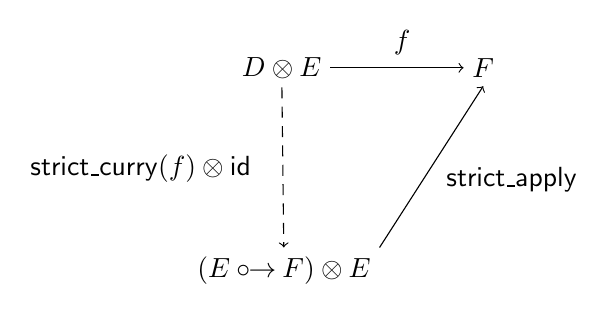
\begin{tikzpicture}[
  x=1cm, y=1cm,
  every node/.style={inner sep=1pt},
  open/.style={circle, draw, fill=white, minimum size=4pt, inner sep=0pt},
  solid/.style={circle, draw, fill=black, minimum size=5pt, inner sep=0pt},
  edge/.style={draw, line width=0.4pt},
  % added for the commutative diagrams: object nodes, and the paper's two
  % arrow kinds -- solid for a named map, dashed for the unique completing map
  obj/.style={inner sep=3pt},
  arrow/.style={draw, line width=0.4pt, ->},
  darrow/.style={draw, line width=0.4pt, ->, dash pattern=on 4pt off 3pt}]

  % vertices
  \node[obj] (dte) at (0.00,2.57) {$D \otimes E$};
  \node[obj] (f)   at (2.56,2.57) {$F$};
  \node[obj] (efe) at (0.03,0.00) {$(E \sfun F) \otimes E$};

  % arrows
  \draw[arrow]  (dte) -- (f);
  \draw[darrow] (dte) -- (efe);
  \draw[arrow]  (efe.north east) -- (f.south);

  % labels printed inside the picture
  \node[anchor=south] at (1.53,2.69) {$f$};
  \node[anchor=east]  at (-0.35,1.29) {\textsf{strict\_curry}$(f) \otimes \textsf{id}$};
  \node[anchor=west]  at (2.05,1.15) {\textsf{strict\_apply}};
\end{tikzpicture}
\end{document}
